\documentclass[aspectratio=169,10pt]{beamer}

\usetheme{metropolis}
\usepackage{appendixnumberbeamer}
\usepackage{booktabs}
\usepackage[scale=2]{ccicons}
\usepackage{pgfplots}
\usepgfplotslibrary{dateplot}
\usepackage{xspace}
\usepackage{tikz}
\usetikzlibrary{mindmap,trees,shapes,arrows,positioning,pie}
\usepackage{tcolorbox}

\title{Understanding the PhD Landscape in Europe and Germany for Computer Science}
\subtitle{Session 1: Embarking on Your CS Doctoral Journey}
\date{\today}
\author{Dr. Bijun Li}
\institute{Expert in International Computer Science Research}

\begin{document}

\maketitle

\begin{frame}{Introduction}
    \begin{itemize}
        \item Growing importance of advanced CS research
        \item Europe as a hub for cutting-edge CS PhD programs
        \item Germany's strengths: strong industry partnerships, excellent funding, world-class research institutions
        \item Comparison with other European countries (e.g., UK, Netherlands, Switzerland)
    \end{itemize}
    
    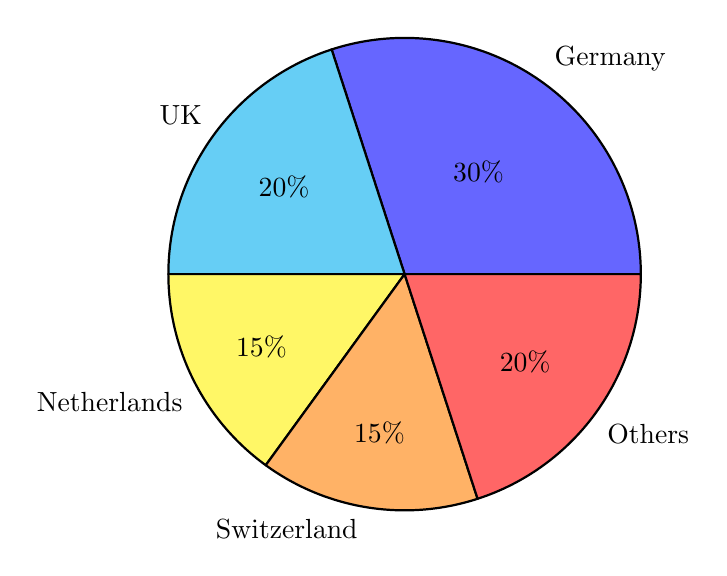
\begin{tikzpicture}
        \pie{30/Germany, 20/UK, 15/Netherlands, 15/Switzerland, 20/Others}
    \end{tikzpicture}
%    \caption{Distribution of top-ranked CS PhD programs in Europe}
\end{frame}

\begin{frame}{European PhD System in Computer Science}
    \begin{columns}[T]
        \begin{column}{0.5\textwidth}
            \textbf{Bologna Process Impact}
            \begin{itemize}
                \item Standardized 3-cycle system
                \item Enhanced mobility within Europe
                \item Focus on quality assurance
            \end{itemize}
        \end{column}
        \begin{column}{0.5\textwidth}
            \textbf{Types of CS PhD Programs}
            \begin{itemize}
                \item Traditional: research-focused
                \item Structured: includes coursework
                \item Industrial: collaboration with companies
            \end{itemize}
        \end{column}
    \end{columns}
    
    \vspace{0.5cm}
    \textbf{Key Differences from Non-European Programs}
    \begin{itemize}
        \item Shorter duration (3-4 years vs. 5-7 years in US)
        \item Less emphasis on coursework
        \item More independent research from the start
    \end{itemize}
\end{frame}

\begin{frame}{Computer Science PhD Landscape in Germany}
    \textbf{Top CS Universities and Research Institutions}
    \begin{itemize}
        \item Technical University of Munich (TUM)
        \item RWTH Aachen University
        \item Max Planck Institute for Informatics
        \item German Research Center for Artificial Intelligence (DFKI)
    \end{itemize}
    
    \textbf{Major CS Research Areas}
    \begin{itemize}
        \item Artificial Intelligence and Machine Learning
        \item Cybersecurity and Cryptography
        \item Quantum Computing
        \item Human-Computer Interaction
        \item Big Data and Data Science
    \end{itemize}
    
    \textbf{Industry Collaborations}
    \begin{itemize}
        \item Strong partnerships with tech giants (e.g., Siemens, SAP, Bosch)
        \item Involvement in Industry 4.0 initiatives
        \item Opportunities for applied research and internships
    \end{itemize}
\end{frame}

\begin{frame}{Application Process for CS PhDs}
    \textbf{Requirements and Eligibility}
    \begin{itemize}
        \item Master's degree in CS or related field
        \item Strong academic record (typically 2.0 or better in German grading system)
        \item Research experience (e.g., master's thesis, publications)
        \item Programming skills and technical proficiency
    \end{itemize}
    
    \textbf{Finding a Supervisor and Research Topic}
    \begin{itemize}
        \item Research faculty profiles and publications
        \item Attend CS conferences and workshops
        \item Leverage online platforms (e.g., ResearchGate, GitHub)
    \end{itemize}
    
    \textbf{Application Documents}
    \begin{itemize}
        \item Research proposal
        \item CV highlighting CS projects and skills
        \item Transcripts and degrees
        \item Letters of recommendation
        \item English proficiency proof (often IELTS 6.5+ or equivalent)
    \end{itemize}
    
    \textbf{Tips for Strong CS PhD Applications}
    \begin{itemize}
        \item Showcase coding projects and GitHub portfolio
        \item Highlight any publications or conference presentations
        \item Demonstrate alignment with potential supervisor's research
    \end{itemize}
\end{frame}

\begin{frame}{Funding Opportunities for CS PhDs}
    \begin{columns}[T]
        \begin{column}{0.5\textwidth}
            \textbf{Types of Funding}
            \begin{itemize}
                \item University positions (often full-time)
                \item DFG Research Training Groups
                \item DAAD scholarships
                \item EU funding (e.g., Marie Skłodowska-Curie)
                \item Industry-sponsored PhDs
            \end{itemize}
        \end{column}
        \begin{column}{0.5\textwidth}
            \textbf{Funding Rates (Monthly, Approx.)}
            \begin{itemize}
                \item University position: €2000-€2500
                \item DFG scholarship: €1365 + allowances
                \item DAAD scholarship: €1200 + allowances
                \item Industry PhDs: Varies, often higher
            \end{itemize}
        \end{column}
    \end{columns}
    
    \textbf{Application Tips}
    \begin{itemize}
        \item Start early: Many deadlines are 6-12 months before program start
        \item Tailor your research proposal to the funding body's priorities
        \item Highlight interdisciplinary aspects of your CS research
        \item Demonstrate potential impact of your work on industry or society
    \end{itemize}
\end{frame}

\begin{frame}{Academic Culture and Expectations}
    \textbf{German Academic Traditions in CS}
    \begin{itemize}
        \item Strong theoretical foundations
        \item Emphasis on methodological rigor
        \item Collaborative research environments
    \end{itemize}
    
    \textbf{Work Culture in German CS Departments}
    \begin{itemize}
        \item Formal communication (use of titles)
        \item High value on punctuality and efficiency
        \item Balance between independent work and team collaboration
    \end{itemize}
    
    \textbf{Expectations for PhD Students}
    \begin{itemize}
        \item Regular progress reports and meetings with supervisors
        \item Participation in departmental seminars and events
        \item Teaching assistance or lab supervision duties
        \item Publication in top-tier CS conferences and journals
        \item Presentation of research at international conferences
    \end{itemize}
    
    \textbf{Publishing and Conferences}
    \begin{itemize}
        \item Focus on conference publications (unlike some other fields)
        \item Aim for top conferences: ICML, NeurIPS, CVPR, SIGCOMM, etc.
        \item Balance between conferences and journal publications
        \item Engage in open-source contributions and code sharing
    \end{itemize}
\end{frame}

\begin{frame}{Building Your Network in CS Academia}
    \textbf{Key CS Conferences and Events}
    \begin{itemize}
        \item Global: ICML, NeurIPS, CVPR, ICCV, SIGCOMM, SIGGRAPH
        \item European: ECML PKDD, ECCV, EuroSys, EuroCrypt
        \item German: KI (German Conference on AI), INFORMATIK
    \end{itemize}
    
    \textbf{Online Platforms and Communities}
    \begin{itemize}
        \item arXiv.org for preprints
        \item GitHub for code sharing and collaboration
        \item Twitter for following researchers and labs
        \item CS-specific forums and discussion boards
    \end{itemize}
    
    \textbf{Networking Strategies}
    \begin{itemize}
        \item Prepare an "elevator pitch" about your CS research
        \item Engage in poster sessions at conferences
        \item Participate in doctoral consortiums
        \item Contribute to open-source projects
        \item Attend summer/winter schools in your CS subfield
    \end{itemize}
\end{frame}

\begin{frame}{Q\&A Session}
    \centering
    \large{Time for Your Questions!}
    
    \vspace{1cm}
    
    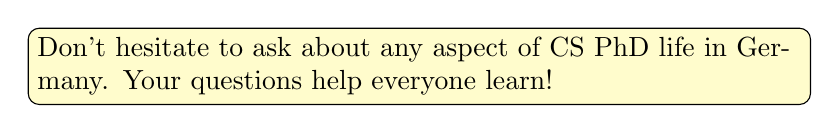
\begin{tikzpicture}
        \node[draw,rounded corners,fill=yellow!20,text width=0.8\textwidth] {
            Don't hesitate to ask about any aspect of CS PhD life in Germany. Your questions help everyone learn!
        };
    \end{tikzpicture}
\end{frame}

\begin{frame}{Preview of Talk 2 and Homework}
    \textbf{Coming Up in Talk 2}
    \begin{itemize}
        \item Detailed financial planning for CS PhDs
        \item Navigating housing and bureaucracy in Germany
        \item Work-life balance in intense CS research environments
        \item Career development and industry connections
    \end{itemize}
    
    \textbf{Homework}
    \begin{itemize}
        \item Research 2-3 potential CS PhD programs or research groups in Germany
        \item Draft an initial research proposal in your area of interest
        \item Create a preliminary budget based on provided funding information
        \item Identify key CS conferences in your subfield and their deadlines
    \end{itemize}
\end{frame}

\end{document}